% Created 2024-06-19 mié 01:51
% Intended LaTeX compiler: pdflatex
\documentclass[presentation]{beamer}
\usepackage[utf8]{inputenc}
\usepackage[T1]{fontenc}
\usepackage{graphicx}
\usepackage{grffile}
\usepackage{longtable}
\usepackage{wrapfig}
\usepackage{rotating}
\usepackage[normalem]{ulem}
\usepackage{amsmath}
\usepackage{textcomp}
\usepackage{amssymb}
\usepackage{capt-of}
\usepackage{hyperref}
\usetheme{Madrid}
\usecolortheme{}
\usefonttheme{}
\useinnertheme{}
\useoutertheme{}
\author{Luis Enrique Perez Señalin}
\date{\textit{<2024-06-19 mié>}}
\title{Proyecto 1 Bimestre}

\hypersetup{
 pdfauthor={Luis Enrique Perez Señalin},
 pdftitle={Proyecto 1 Bimestre},
 pdfkeywords={},
 pdfsubject={},
 pdfcreator={Emacs 27.1 (Org mode 9.3)}, 
 pdflang={Spanish}}
\begin{document}

\maketitle
\begin{frame}{Outline}
\tableofcontents
\end{frame}


\section{Funciones Utilizadas}
\label{sec:orga2c70d9}

\begin{frame}[label={sec:org8be4009}]{Función entero a binario}
Entero a binario:
\begin{center}
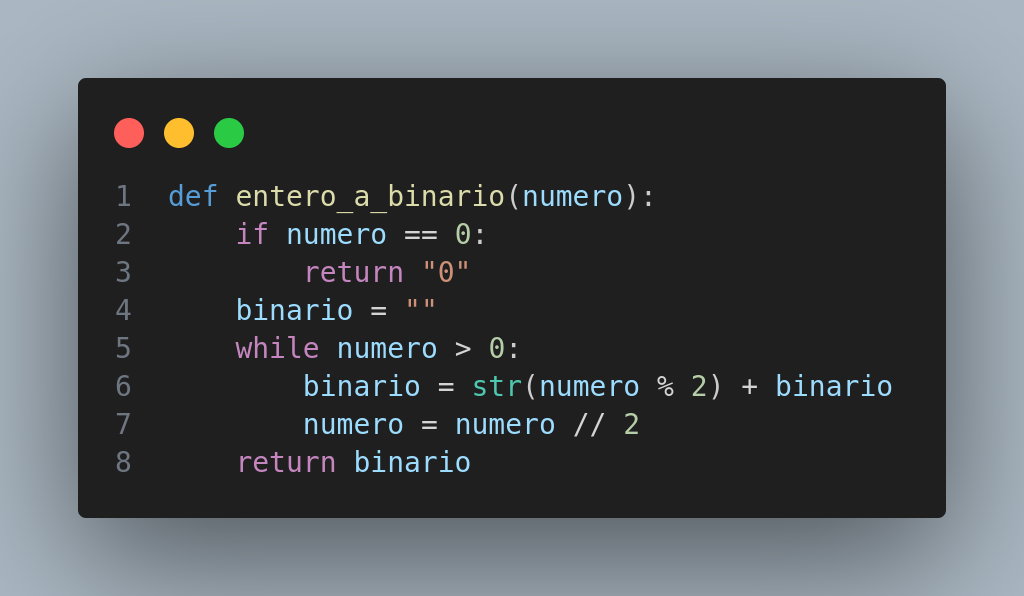
\includegraphics[width=.9\linewidth]{./img_codigo/entero_binario.png}
\end{center} 
\end{frame}

\begin{frame}[label={sec:orgf1562c5}]{Funcion fraccion a binario}
Fraccion a binario:
\begin{center}
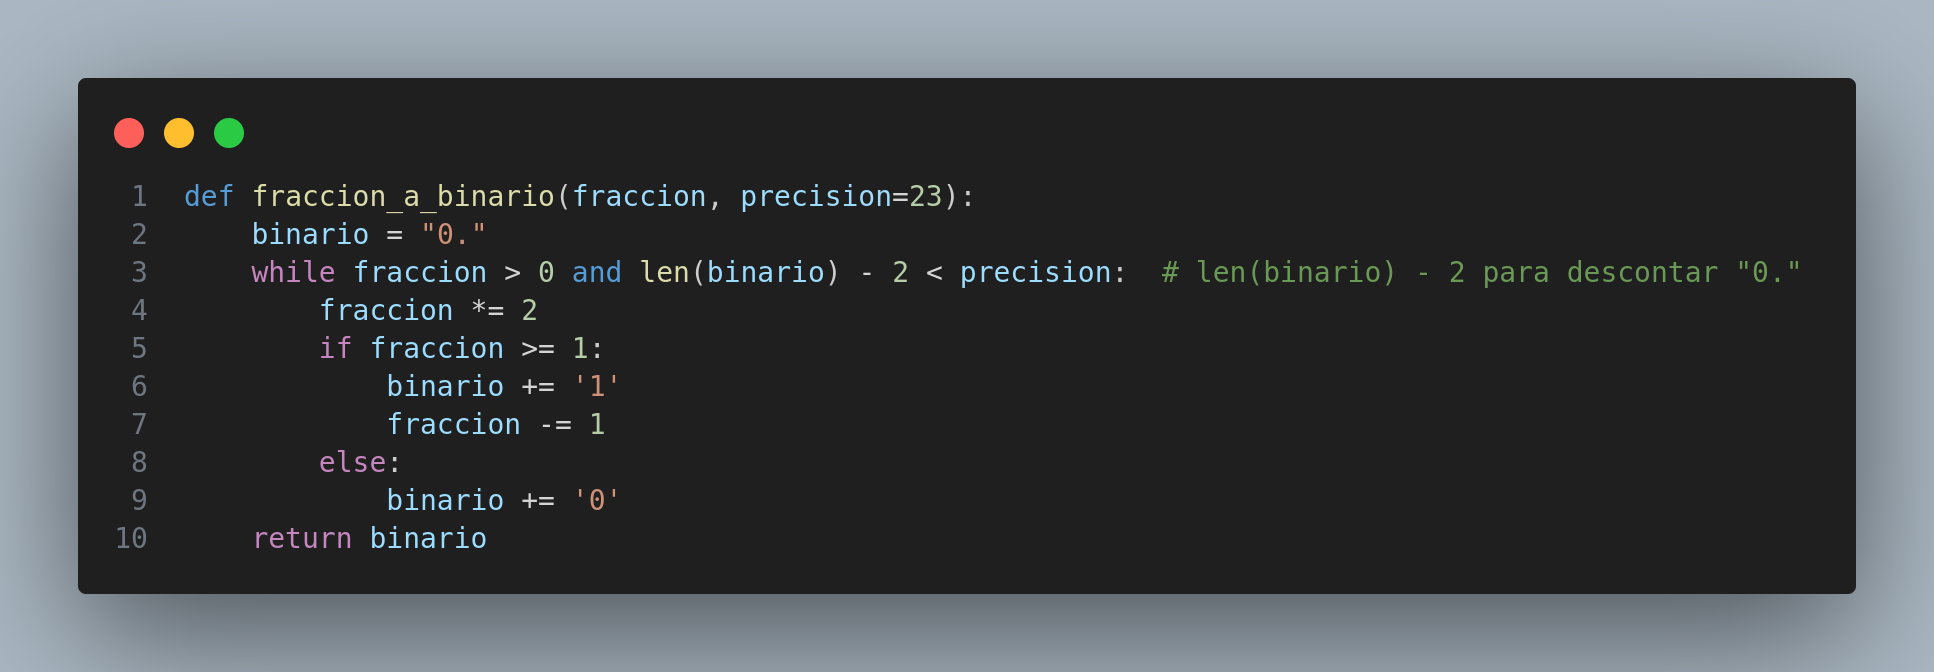
\includegraphics[width=.9\linewidth]{./img_codigo/fraccion_binario.png}
\end{center} 
\end{frame}

\begin{frame}[label={sec:org4fb1597}]{Calculo Exponente}
Funcion retorna exponente y binario normalizado

\begin{center}
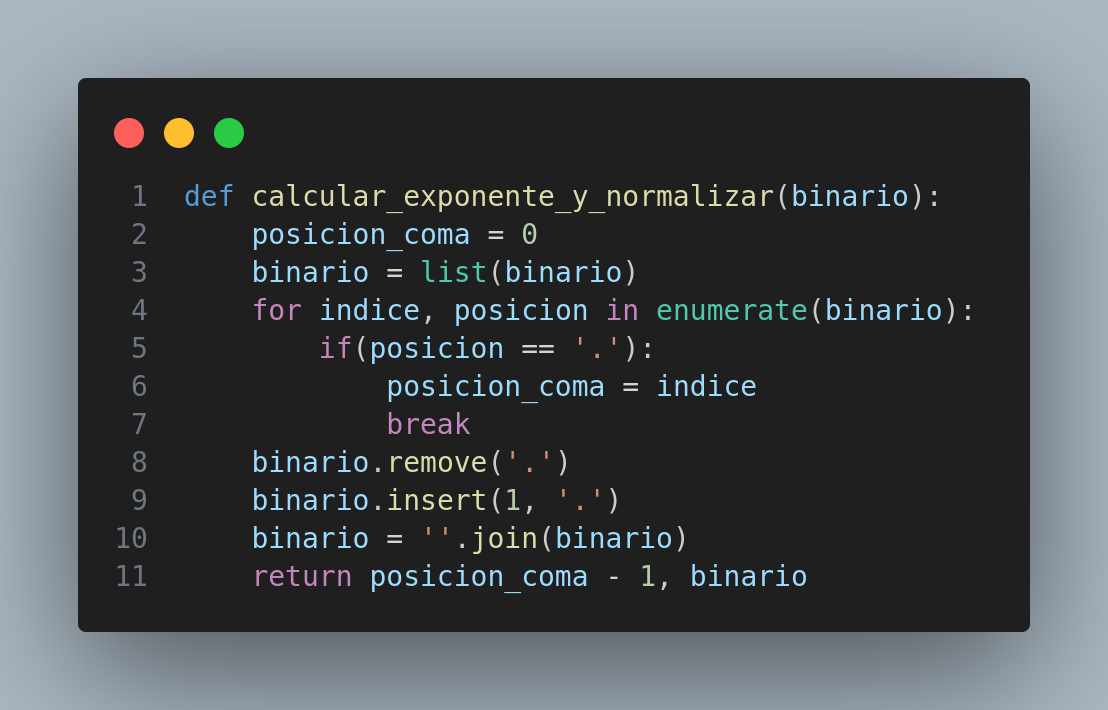
\includegraphics[width=.9\linewidth]{./img_codigo/calculo_exponente.png}
\end{center}
\end{frame}

\begin{frame}[label={sec:orgcc64585}]{Calculo Mantisa}
Funcion que calcula la mantisa
\begin{center}
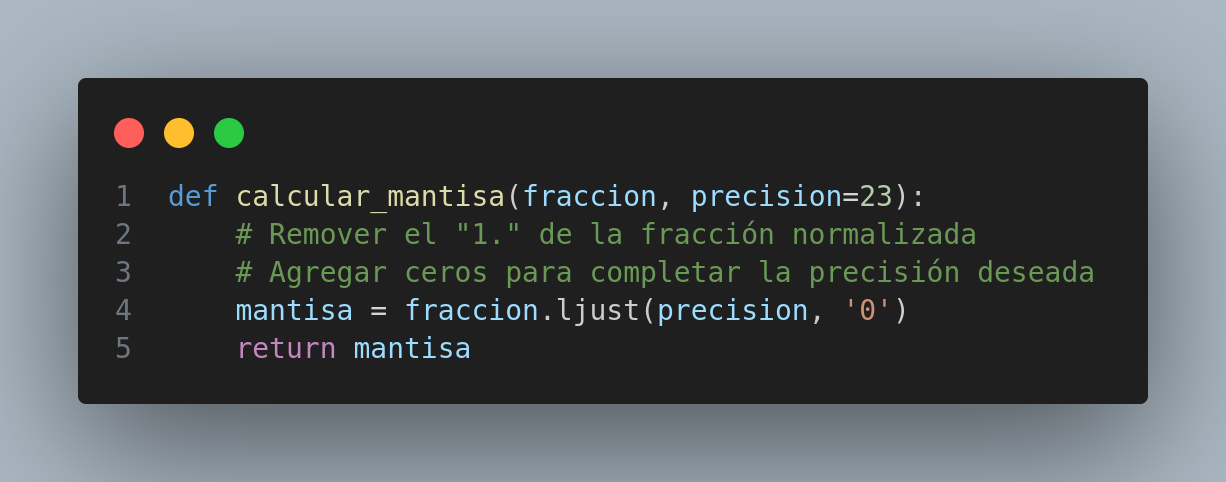
\includegraphics[width=.9\linewidth]{./img_codigo/calculo_mantisa.png}
\end{center} 
\end{frame}

\begin{frame}[label={sec:orgdeb9c15}]{Llamado a la funcion}
Llamado del codigo:

\begin{center}
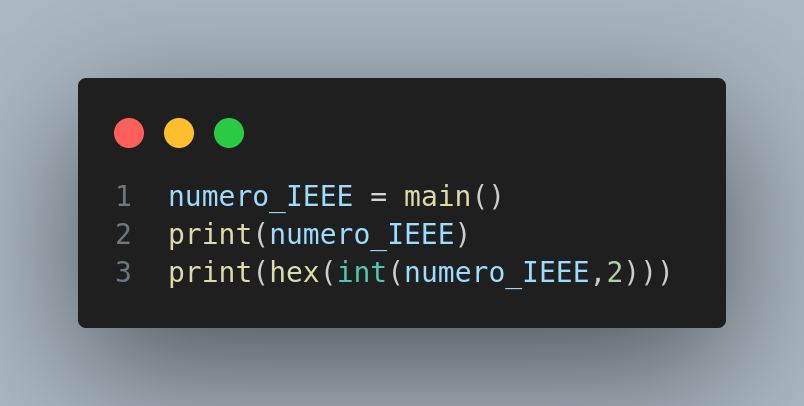
\includegraphics[width=.9\linewidth]{./img_codigo/llamado_funcion.png}
\end{center}
\end{frame}
\end{document}
